\documentclass[11pt]{article}
\usepackage{geometry}
\geometry{
 a4paper,
 total={210mm,297mm},
 left=20mm,
 right=20mm,
 top=20mm,
 bottom=20mm,
 }
 
\usepackage[english]{babel}
\usepackage[utf8x]{inputenc}
\usepackage{amsmath}
\usepackage{graphicx}
\usepackage[table,xcdraw]{xcolor}
\usepackage[colorinlistoftodos]{todonotes}
\usepackage{multicol}
\usepackage{ragged2e}
\usepackage{tocloft}
\usepackage{titlesec}
\usepackage{natbib}
\usepackage[parfill]{parskip}
\usepackage{amssymb}
\usepackage{textcomp}
\usepackage{float}
\floatstyle{plain}
\usepackage{color}
\usepackage{epstopdf}
\usepackage{hyperref}
\usepackage{comment}
\hypersetup{
    colorlinks=true,
    linkcolor=blue,
    filecolor=magenta,      
    urlcolor=cyan,
    citecolor=blue
}
\urlstyle{same}
\usepackage{fancyhdr}
\usepackage{lipsum}
\usepackage{subscript}
\usepackage{siunitx}
\usepackage[hypcap]{caption}
\usepackage{capt-of}
\usepackage{wasysym}
\usepackage{wrapfig}
\usepackage{enumitem}
\usepackage{pdflscape}
\usepackage{pdfpages}
\usepackage{csquotes}
\usepackage{mathtools}

%making the bloody title 
\makeatletter
\renewcommand{\maketitle}{\bgroup\setlength{\parindent}{0pt}
\begin{flushleft}
  \textbf{\@title} %the empty line is impt

  \@author
\end{flushleft}\egroup
}
\makeatother

%random things needed
%\renewcommand{\cftsecleader}{\cftdotfill{\cftdotsep}} %let the content table have dots to number
\linespread{1.5}  %making one and a half spacing-sh one and half is actually 1.3
\frenchspacing
%\titlespacing\subsection{0pt}{12pt plus 4pt minus 2pt}{0pt plus 2pt minus 2pt} 
\titlespacing\subsubsection{0pt}{12pt plus 4pt minus 2pt}{0pt plus 2pt minus 2pt} %less spacing between subsubsections
\pagestyle{fancy}
% Set the right side of the footer to be the page number
\fancyhf{} % sets both header and footer to nothing
\renewcommand{\headrulewidth}{0pt}
\fancyfoot[R]{\thepage}
\fancypagestyle{plain}{%
    \renewcommand{\headrulewidth}{0pt}%
    \fancyhf{}%
    \fancyfoot[R]{\thepage}%
}
\setlength{\parskip}{0pt}
%make modulus same length as text, starred makes it shorter
\DeclarePairedDelimiter\abs{\lvert}{\rvert}%
\DeclarePairedDelimiter\norm{\lVert}{\rVert}%

%insert title
\title{\textbf{\LARGE{BEEquations \& test reasons}}}
\smallskip
\date{} 
\author{%
\large{Lim Jia Le}
}

\begin{document}
\maketitle
\smallskip
\tableofcontents

\section{Dissimilarity Measures}

Metaweb: Regional pool of species and all interactions. ($\gamma$ diversity) \\
Realisation: Local network drawn from regional metaweb ($\alpha$ diversity) \\
$\beta$ diversity: Differences between two subsets/realisations/local networks\\

\underline{Whittaker's $\beta$ diversity measure~\citep{Poisot2012}}

The `realisation membership' vetor, $M$, takes the form:
\begin{flalign}
M &= [c = \norm{A\notin B}, b =  \norm{B\notin A}, a = \norm{A\cup B}] &
\end{flalign}
Basically: 
\begin{itemize}
	\item c is the number of items unique to realisation $A$
	\item b is the number of items unique to realisation $B$
	\item a is the number of items common to both realisations.
	\item items can refer to species, interactions, etc...
\end{itemize}
\begin{flalign}
	\boldsymbol{ \beta_{w}}(M) & = \frac{a + b + c}{(2a + b + c)/2} - 1 &
\end{flalign}
\begin{flalign}
	\beta_{WN} & = \beta_{ST} + \beta_{OS} &
\end{flalign}
where:
\begin{itemize}
	\item $\beta_{WN}$: Dissimilarity of interactions ($\beta_{int}$ in~\cite{CaraDonna2017})
	\item $\beta_{ST}$: Dissimilarity of interactions due to species turnover ($\beta_{WN} - \beta_{OS}$)
	\item $\beta_{OS}$: Dissimilarity of interactions established between species common to both realisations (interaction rewiring; $\beta_{rw}$ in~\cite{CaraDonna2017}; extract common species of both networks, number of interactions common to both networks, a and unique to each, b \& c)
\end{itemize}

$\beta_{S}$: Dissimilarity in the species composition of communities
 $\boldsymbol{ \beta}$ ranges from 0 to 1. \\
 A higher $\boldsymbol{ \beta}$ reflects a higher difference between two realisations. \\
 \newpage

\begin{figure}[h]
  \centering
    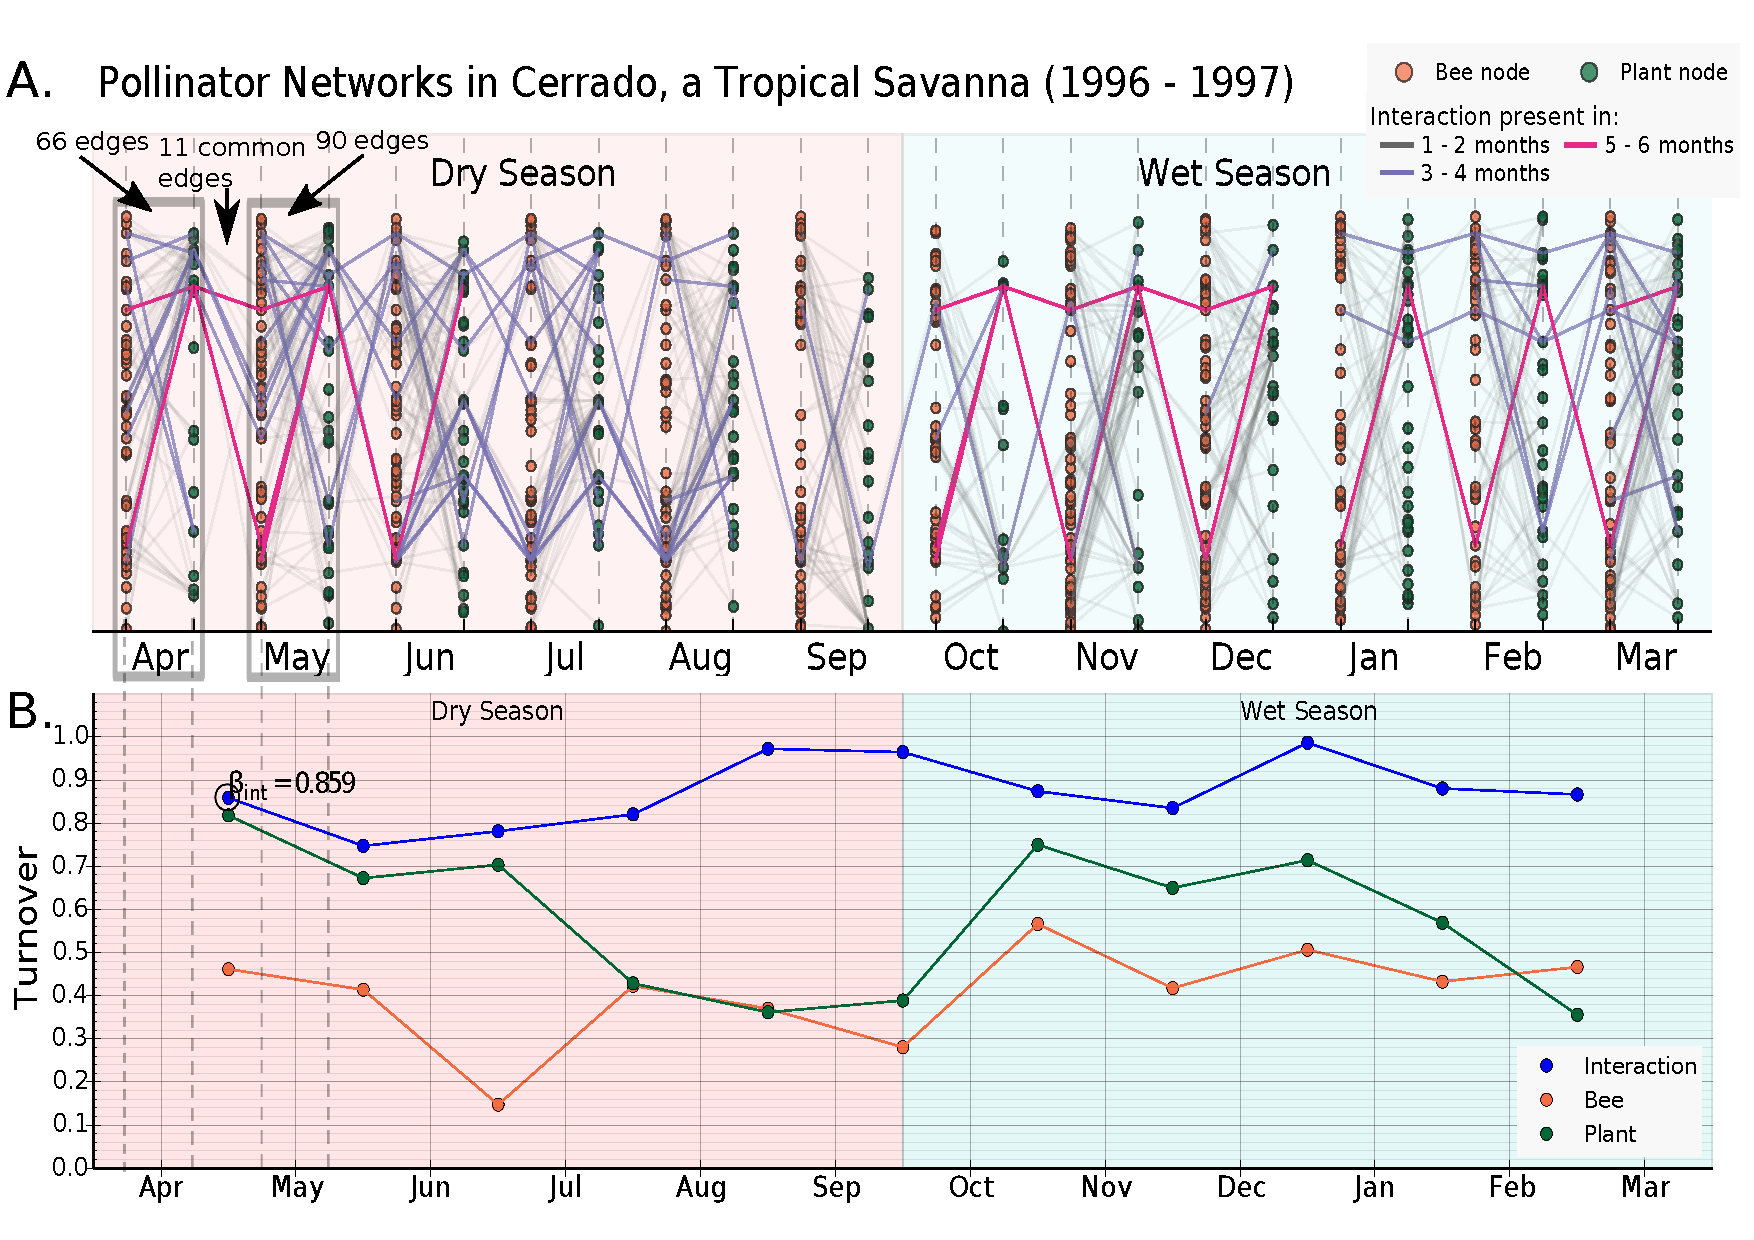
\includegraphics[width=\textwidth]{PosterFigure.pdf}
  \captionof{figure}{(A) Monthly bee pollinator networks from April 1996 to Mar 1997. \\
(B) Bee-flower interaction turnover and species turnover from April 1996 to Mar 1997. \\
 Average monthly precipitation sum = 25.3 mm (Dry Season), 239.6mm (Wet Season) \\}
   \label{fig:posterfigure}
\end{figure}

For example, when comparing between April and May networks in \autoref{fig:posterfigure}:
\begin{flalign}
     \beta_{WN} & = \frac{11 + 55 + 79}{(2\times11 + 55 + 79)/2} - 1 \quad = 0.859 &\\
     \beta_{OS} & =  have to find list of common species, extract interactions between only common species than run turnover script....hmm&\\
     \beta_{ST} & = \beta_{WN} - \beta_{OS} = 0.859 -  &\\ 
\end{flalign} 

\underline{Multi-site dissimilarity~\citep{Poisot2012}} \\
A measure of global variability between the different realizations, assuming system is sampled enough, and metaweb a prozy of the regional pools of species and interactions.

Connectance is $L/n^{2}$, where $L$ is number of interactions and $n$ is number of species.

Nope, I don't understand. (Understand the idea but not the equations.)

\section{Statistic test}

\subsection{Spearman's correlation coefficient}
Non-parametric measure of rank correlation. \\
\underline{x vs. $\beta_{WN}$} \\
How much x explains/correlates with $\beta_{WN}$. \\
How much x is responsible for interaction turnover.
\underline{x vs. $\beta_{OS}$} \\
How much x explains/correlates with $\beta_{OS}$. \\
How much x is responsible for interaction rewiring among common species. \\
\underline{x vs. $\beta_{ST}$} \\
How much x explains/correlates with $\beta_{ST}$. \\
How much x is responsible for interaction turnover due to species turnover. \\
\underline{x vs. $\beta_{S}$}
How much x explains/correlates with $\beta_{S}$. \\
How much x is responsible for species turnover. \\
\\
\underline{Random shuffling } \\
Spearman coefficient compare with mean of distribution (of coefficients generated from Monte Carlo stimulation) \\
$H_{0}$: By random chance, x correlated with y. \\
$H_{a}$: Higher than mean-> how to determine how much higher, Not random, x probably a driving force of y. (What do you mean by systemic?) \\
What if it is lower than mean... play a smaller role than if random...? or not possible scenerio....?\\
Where x \& y pairs:
\begin{itemize}
	\item $\beta_{ST}\quad vs.\quad \beta_{WN}$
	\item $\beta_{OS}\quad vs.\quad \beta_{WN}$
	\item $\beta_{S}\quad vs.\quad \beta_{WN}$
	\item $\beta_{S}\quad vs.\quad \beta_{ST}$
	\item climate turnover vs. $\beta_{S}, \beta_{ST}, \beta_{OS}, \beta_{WN}$
	\item what about temperature turnover? only for shuffling species within seasons, within years, everything?
	\item also, shuffle Cerrado and BoaVentura separately right?
\end{itemize}

\underline{Random shuffling of interactions within months} \\
Ignore climate turnover vs. $\beta_{S}$ \\

\underline{Random shuffling of species within seasons} \\
\underline{Random shuffling of species within year} \\
\underline{Random shuffling of species across all} \\


\newpage
\bibliography{BEEquations}
\bibliographystyle{cell}

\end{document}


